\addcontentsline{toc}{chapter}{Занятие 5. Винеровский процесс}
\chapter*{Занятие 5. Винеровский процесс}

\addcontentsline{toc}{section}{Контрольные вопросы и задания}
\section*{Контрольные вопросы и задания}

\subsubsection*{Приведите определение процесса Пуассона.}

$\left\{ N \left( t \right), \, t \geq 0 \right\} $ --- процесс Пуассона, если
\begin{enumerate}
  \item $N \left( 0 \right) = 0$;
  \item при $t_1 < t_2 < \dotsc < t_n$ события
  $$N \left( t_1 \right), N \left( t_2 \right) - N \left( t_1 \right), \dotsc,
    N \left( t_n \right) - N \left( t_{n - 1} \right) $$
  --- независимые;
  \item число событий на интервале зависит только от длины интервала,
  то есть есть однородность приращений
  $$N \left( t + s \right) - N \left( t \right) \overset{d}{=}
    N \left( s \right) \sim
    Pois \left( \lambda s \right).$$
\end{enumerate}

\subsubsection*{Запишите конечномерные распределения процесса Пуассона.}

Одномерные распределения
$$P \left\{ N \left( t \right) = k \right\} =
  e^{-\lambda t} \cdot \frac{ \left( \lambda t \right)^k}{k!}.$$

Двумерные распределения: $t_1 < t_2$.
Перейдём к приращениям
$$P \left\{ N \left( t_1 \right) = k_1, \, N \left( t_2 \right) = k_2 \right\} =
  P \left\{
    N \left( t_1 \right) = k_1, \, N \left( t_2 \right) - N \left( t_1 \right) = k_2 - k_1
  \right\} =$$
Случайная величина $N \left( t_1 \right) \sim Pois \left( \lambda t_1 \right) $, а
$N \left( t_2 \right) - N \left( t_1 \right) \sim
  Pois \left( \lambda \left( t_2 - t_1 \right) \right) $.
Совместная вероятность --- это произведение вероятностей
$$= e^{-\lambda t_1} \cdot \frac{ \left( \lambda t_1 \right)^{k_1}}{k_1!} \cdot
  e^{-\lambda \left( t_2 - t_1 \right) } \cdot
  \frac{ \left( \lambda \left( t_2 - t_1 \right) \right)^{k_2 - k_1}}{ \left( k_2 - k_1 \right)!}.$$

\subsubsection*{Какой вид имеют траектории процесса Пуассона?}

Траектория изображена на рисунке \ref{fig:3}.

\begin{figure}[h!]
  \centering
  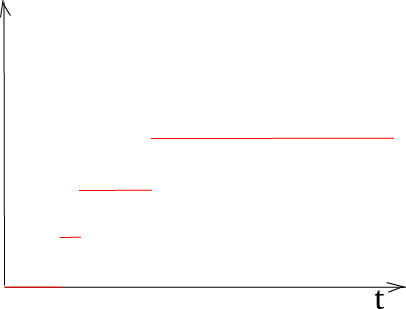
\includegraphics[width=.4\textwidth]{./pictures/3.png}
  \caption{График пуассоновского процесса}
  \label{fig:3}
\end{figure}

\subsubsection*{Какое содержание имеет параметр процесса Пуассона?}

$N \left( t \right) $ --- число событий, произошедших до момента времени $t$.
